% !TEX root = Formulaire_Fluides.tex

%\appendix












%\pause

%\addcontentsline{toc}{section}{B. Diagramme de Moody}
\clearpage
\section{Pertes de charges et Diagramme de Moody}
$$
\Delta P = \frac{\rho U^2 L}{D} \lambda(Re,\epsilon)
$$

$$ 
Re = \frac{U D}{\nu}, \quad \epsilon = \frac{k}{D}
$$

\begin{description}
\item[Régime laminaire ($Re \leq 2000$) ]:

Pour $Re < 2000$ on peut utiliser la formule de Poiseuille :

$$
\lambda = \frac{64}{Re}
$$
\item[Régime turbulent  ($Re \geq 2000$) ]:


Pour $\varepsilon < 0.01\%$ et $Re<10^5$ on peut utiliser  la formule de Blasius : 
\begin{equation}
   \lambda= 0.316 \, Re^{-1/4}
 \end{equation}

Pour $Re >4000$ et $\epsilon$ quelconque, on utilise généralement la formule de Colebrook (semi-explicite) :

\begin{equation}
  \frac{1}{\sqrt{\lambda}} = -2 \log_{10} \left (
  \frac{2.51}{Re\sqrt{\lambda}} + \frac{\varepsilon}{3.71}
  \right)
\end{equation}
\end{description}



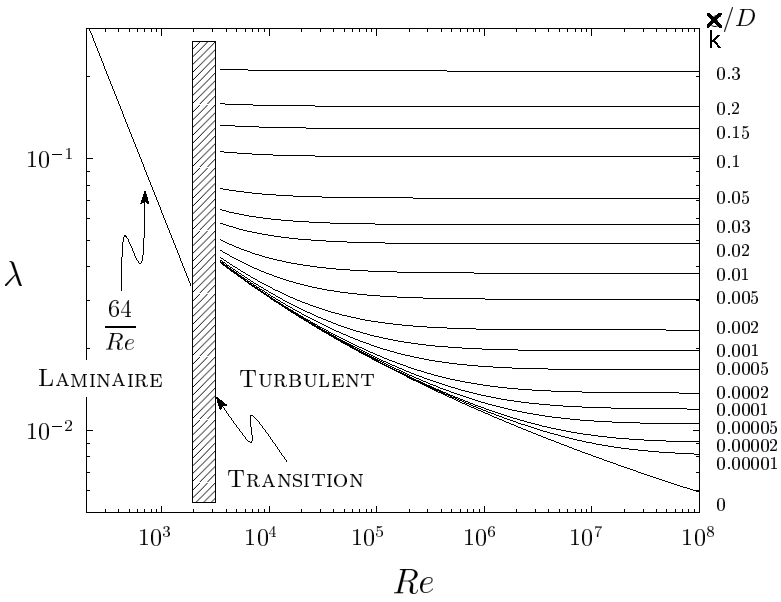
\includegraphics[width=\linewidth]{../FIGURES/Moody_diagram.pdf}


\addcontentsline{toc}{section}{H. Ecoulement compressible isentropique de gaz parfait}
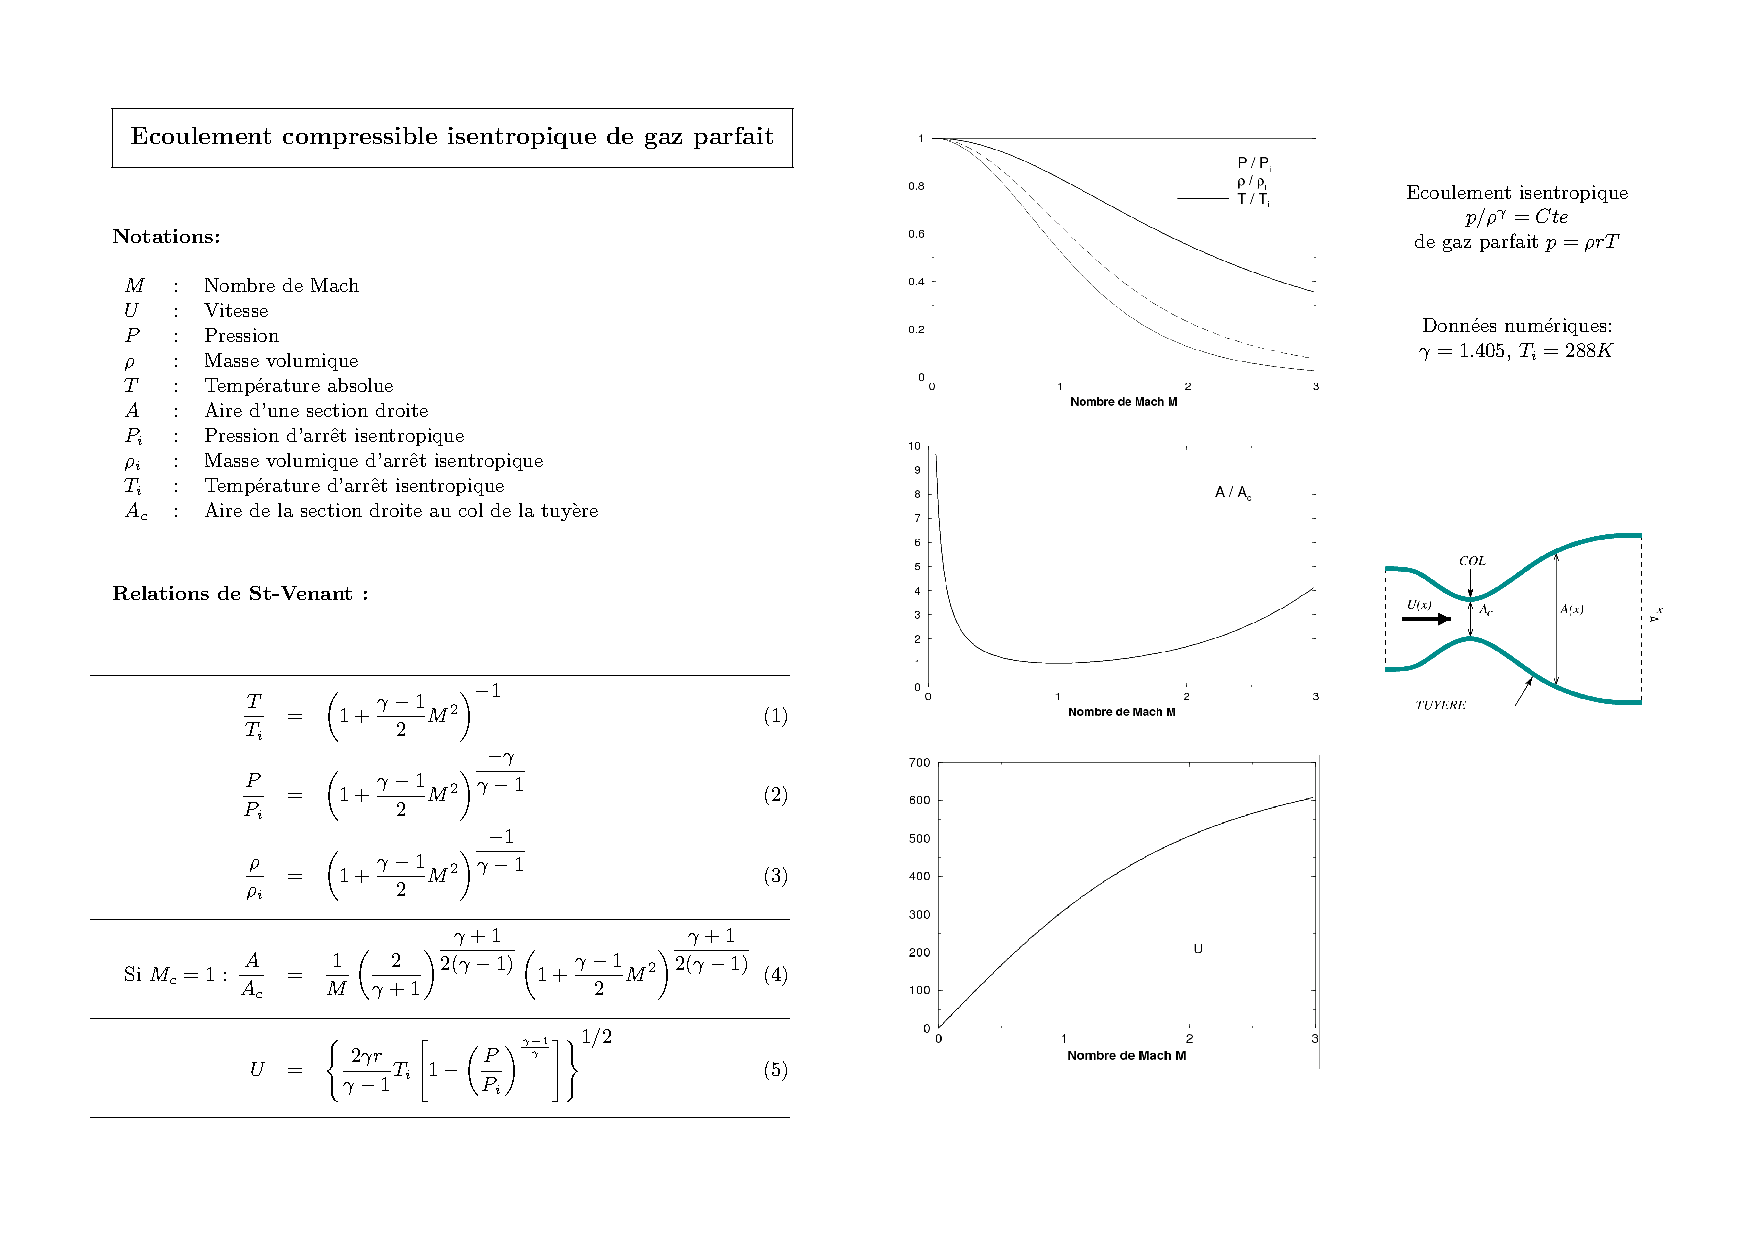
\includepdf[pages=1-2, landscape]{./Figures/St_Venant.pdf}

\addcontentsline{toc}{section}{I. Relations de saut a travers un choc droit}
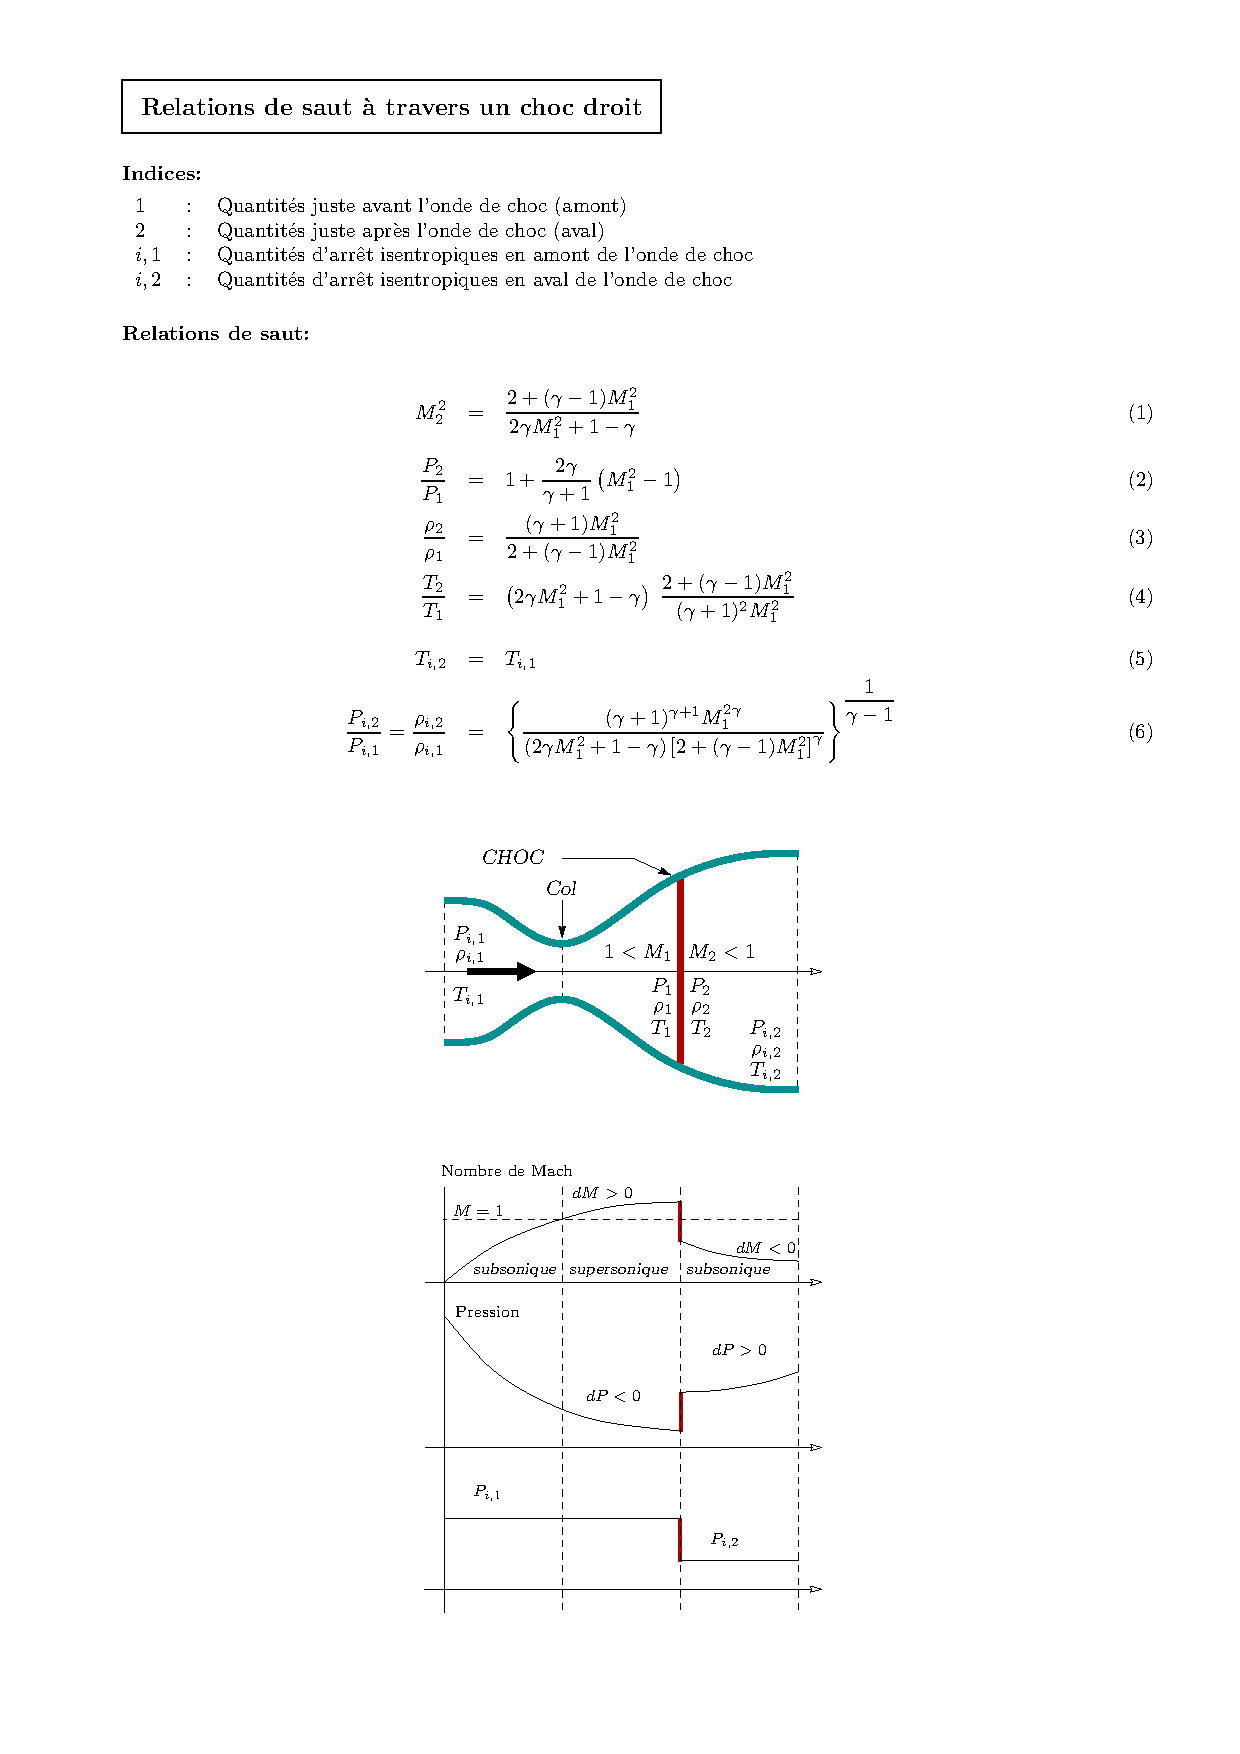
\includepdf[pages=1-2]{./Figures/choc.pdf}